\chapter{Methodology} % Main chapter title

\section{Complex networks}

Many real systems are composed of a large number of elements interacting with each other. Due to interactions, without any central force, the system exhibits the emergence of collective behaviour on the macro level. Such a system is called a Complex System and its properties can not be predicted from the behaviour of the one individual. An example of a complex system is the human brain. The structure of the brain network and its properties are fundamental for brain functioning, while an emergent phenomenon is a human intelligence. In societies, people's interactions lead to civilization, economy, formation of social groups. Also, the animal populations show different levels of organization that emerge from the individual's interactions. \cite{boccaletti2006complex} %latorro

The research in complex systems focuses on the structure of the interactions between units. Knowing how branches of the system are connected, we can determine the emergence of the collective behaviour of the system. For the brain network, we can construct representation with neurons and synapses, representing the brain connectivity. Neurons in the same brain area are closely connected \cite{caldarelli2018complex}. Similarly, we can define communication between people. The structure of these interactions gives us insights, for example, how information propagates through the system. The presence of people with many connections can lead to faster information flow. 

Despite the differences between complex systems, they can be studied using complex networks; with sets of nodes (vertices) and links (edges). Elements in the system are nodes, while interactions between them are given as edges. This approximation allows us to treat equally social (graph of actors), biological (network of proteins) or even technological systems (internet, traffic). \ In recent years, complex network theory has application in different fields, and the availability of big data incurs its development. \cite{costa2011analyzing} \cite{costa2007characterization}\\
%Analyzing and Modeling Real-World Phenomena with Complex Networks: A Survey of Applications
%Characterization of Complex Networks: A Survey of measurements

The complex network theory originates from the graph theory in mathematics. %These days, the graph and network are used as equivalent terms. 
The first mathematical problem solved using graph theory was $Konigsberg$ problem of seven bridges. The city $Konigsberg$ had seven bridges connecting the city's parts across the river and the island in the middle. The question was, is it possible to find a walk that crosses all seven bridges only once. Representing the problem as a graph, as in figure \ref{fig:Krgraph}, Euler managed to simplify the problem; the parts of the land are represented as nodes while bridges between them are links. Crossing each bridge only once is possible if each part of the land has an even number of connections. By this it is possible to enter one part of the land from one bridge and leave it by the other. As each node has odd number of connections, in this case it is not possible, see Fig. \ref{fig:Krgraph}.

\begin{figure}[h!]
	\centering
	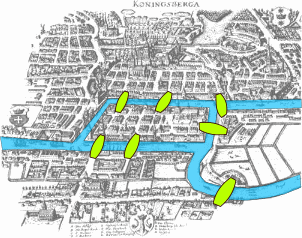
\includegraphics[width=0.3\linewidth]{Figures/Konigsberg_bridges.png} \hspace{2cm}
	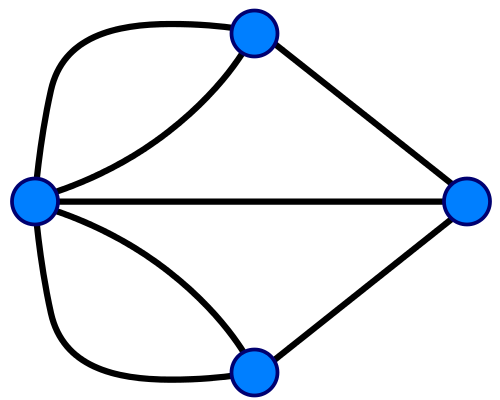
\includegraphics[width=0.3\linewidth]{Figures/Konigsberg_graph.png}
	\caption{The Kronigsber problem of seven bridges.}
	\label{fig:Krgraph}
\end{figure}

\section{Types of networks}

%The seven bridges problem in Fig. \ref{fig:Krgraph} is represented with the \textbf{simple network} structure. 
The graph or network $G$ is defined as $G=(\boldsymbol{V}, \boldsymbol{E})$, where $\boldsymbol{V} = \{ v_1, v_2, ... v_N\}$ is a set of $N$ nodes (vertices), and  $\boldsymbol{E} = \{e_1, .. e_L\}$ is a set of $L$ edges (links). The edge is pair of nodes $e = (v_i, v_j), $ such that $\{v_i,v_j\}\in \boldsymbol{V}$. The most basic network representation considers \textbf{unweighted and undirected} structure. The edges are unweighted, meaning that all interactions in the network are equally important.  Because network is un-directed, edges are symmetric, such that $(v_i, v_j)$ implies $(v_j, v_i)$. In \textbf{directed} networks this simmetry is broken. The interaction between two nodes $v_i$ and $v_j$, can be only in one direction. A typical example is World Wide Web, where webpages are nodes and hyperlinks are directed edges. In biological networks, gene regulation and neural activation can be described as directed network. The first column a) in Figure \ref{fig:graph_dir} shows the graphical representation of two networks with equal number of nodes; the first one is underected and the second one is directed. 


Even though, graphical representation can be useful for describing the network structure, mathematical representation allow us to characterize the statistical properties of the networks. The graph $G$, with $N$ nodes could be represented with \textbf{adjacency matrix} $|A| = N \times N$ \cite{boccaletti2006}. The elements of the matrix are positive if there is connection between two nodes $v_i$ and $v_j$. 
\begin{equation}
A_{ij} =
\begin{cases}
1 & \text{ ($v_i$, $v_j$) $\in$ $E$}\\
0 & \text{ ($v_i$, $v_j$) $\notin$ $E$}
\end{cases}       
\end{equation}

The column b) on Figure \ref{fig:graph_dir} shows adjacancy matrix representation of given graphs. By convention diagonal elements $A_{ii}=0$, as self-loops are not allowed. For undirected network adjacency matrix is symmetric $A_{i,j}=A_{ji}$, but in the case of directed network matrix is not symmetric, as edges are drawn in one direction only. The number of edges and nodes are dependent variables. Considering that each node can make $N-1$ connections, the maximum number of the edges in the network is $L_{max}=N(N-1)/2$, as each edge is counted twice. For directed network it is possible to draw $L_{max}=N(N-1)$ edges.  

\begin{figure}[h!]
\centering
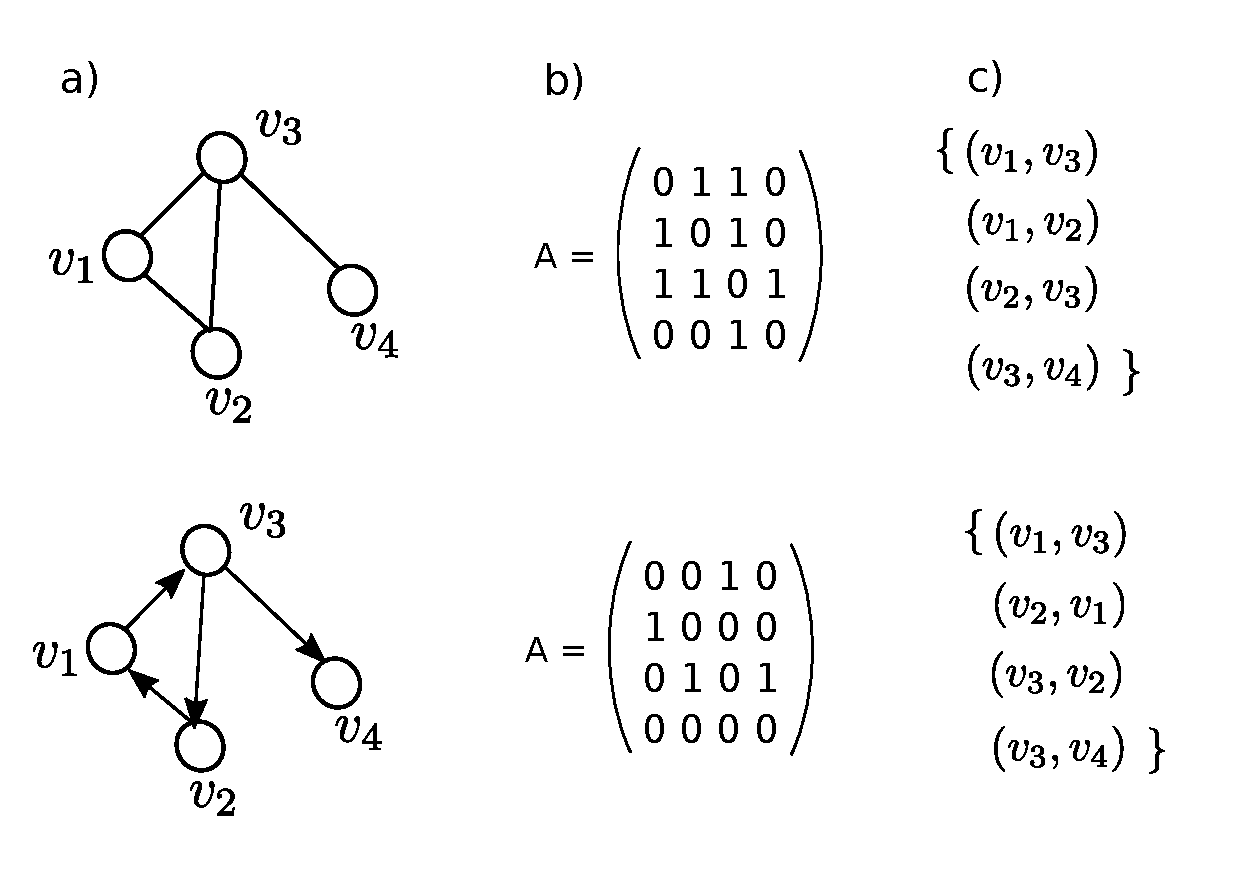
\includegraphics[width=0.8\linewidth]{figures/methodology/directed_graph.pdf} 
\caption{a) Graph representation of undirected (top panel) and directed (bottom panel) network. The same networks are represented with adjacency matrices column b), and edge list representation in column c).}
\label{fig:graph_dir}
\end{figure}

When it comes to the large network structure, it is common to represent the graph as edge list. In this case, illustrated on Figure \ref{fig:graph_dir}, column c), graph is described with the list of links that are in the graph, $G = \{ \{v_i,v_j\}\}$. To distinguish between undirected and directed structures, for undirected representation it is possible writing two edges $(v_i, v_j)$ and $(v_j, v_i)$, otherwise in the computational algorithm should be specified if the edges are considered symmetric or not.



%Other equivalent way of representing graph is as edge list. Instead of having adjacency matrix, graph is described with the list of links that are in graph. The graph is then pair of $N, g$, where N is set of nodes, and $g$ is collection of links, listed as subset of $N$ of size 2. So the network is written as $g = \{ \{1,2\}, \{2,3\}\}$.


%On the other hand, in the \textbf{weighted} networks, edges are assigned with different values. This representation help us to distinguish between   

%The specific properties of the nodes are also neglected in this representation. The \textbf{adjacency matrix} ${A} = N \times N$ has value $1$ if there is connection between two nodes, otherwise it is $0$ \cite{boccaletti2006}\\

%For example, if we consider unweighted, undirected network, with only 3 nodes and two connections, adjacency matrix is:


%\begin{equation}
%A = \begin{bmatrix}
%0 & 1 & 1\\
%1 & 0 & 0 \\
%1 & 0 & 0 \\
%\end{bmatrix}
%\end{equation}

%The self loops usually are not considered, meaning that $A_{ii}=0$. 
%The complex system can be represented by complex network $G=(V, E)$, where the elements of system (atoms, proteins, people) map to set of $N$ nodes $V=\{1, 2, ...,N\}$. The interactions between elements map to $L$ links between nodes, $E = \{ e_1, e_2... e_L\}$. The \textbf{adjacency matrix} ${A} = N \times N$ has value $1$ if there is connection between two nodes, otherwise it is $0$ \cite{boccaletti2006}.

To create the more realistic models, sometimes it is essential to include the specific properties of the system in the network representation. For example, to emphasis the frequent interactions between nodes, edges can be assigned with different values, such networks are \textbf{weighted}. They can be described with adjacency matrix, whose elements can take any real number $A_{ij}=w_{ij}$ and $w_{ij}>0$. In general edges may be associated with any categorical variable. Similarly additional properties can be added to nodes, or even to the whole network structure. To include the \textbf{temporal} component in the network, edges or nodes may be characterized with the time, when the interaction happen. Finally, if two nodes interact in different ways, the \textbf{multigraph} is appropriate configuration where multiply edges are allowed. The graphical representation of discussed network representations is given on the Figure \ref{fig:multigraph}.    

\begin{figure}[h!]
	\centering
	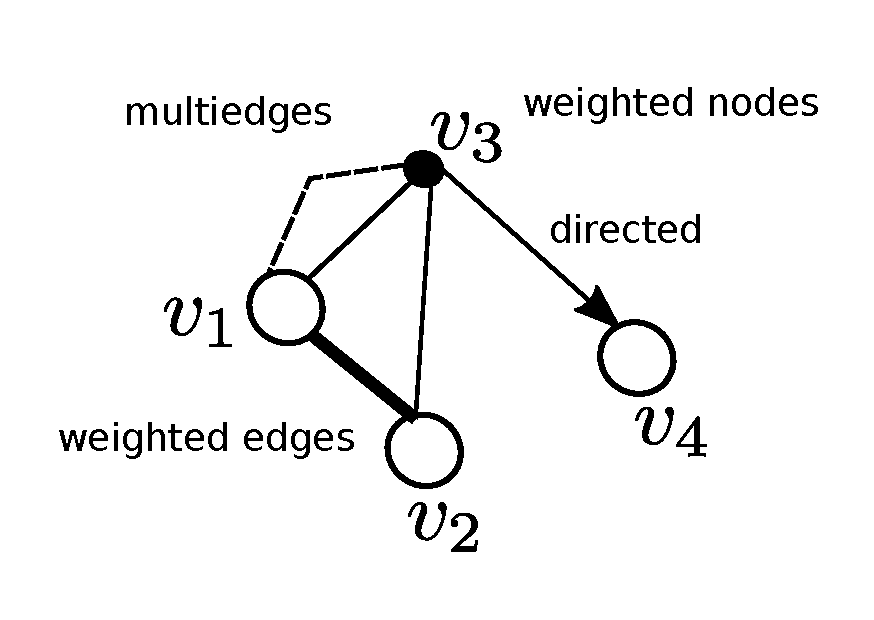
\includegraphics[width=0.4\linewidth]{figures/methodology/multi_graph.pdf} 
	\caption{The complex networks may represent different characteristics of the system. The edges can be directed, weighted or multiply. Also nodes can be assigned with different weights or any relevant feature.}
	\label{fig:multigraph}
\end{figure}

%Sometimes it is essential to include specific properties of the system in the network representation, which can help create more realistic models. The additional properties can be added on the edge, node or network level.

%The edges may be signed, representing activation in the biological system or trust and distrust in the social system. In general, edges can be associated with any categorical variable. If attribute describes the time when an interaction between nodes happened; network is called \textbf{temporal}. Finally, \textbf{multigraph} allows the presence of multiply edges between two nodes. For the network between cities, edges may be different driving paths between them. In neuron cells, multiply synapses are represented as distinct edges. \\















